\documentclass[10pt, titlepage]{report}

\usepackage[utf8]{inputenc}
\usepackage[T1]{fontenc}
\usepackage[francais]{babel}

%Caractères spéciaux

\usepackage{lmodern}
\usepackage{amsmath}
\usepackage{amssymb}
\usepackage{mathrsfs}

\usepackage{eurosym} %insertion signe euro
\usepackage{graphicx} %insertion d'images
\usepackage{fancyhdr} %en-tete et pied de page

\title{\bsc{cahier des charges}\\Projet flight arena}
\author{mr cube :\\
Vincent \bsc{Rospini-Clerici},\\
Guillaume \bsc{Rebut}\\
%Nikolas \bsc{Miletic}\\
chef de projet : Arthur \bsc{Remaud}}
\date{16 janvier 2015}

\pagestyle{fancy}
\fancyhead{}
\fancyfoot{}
\lhead{Cahier des charges}
\rhead{Projet Flight Arena}
\lfoot{mr cube}


\begin{document}

\maketitle

\renewcommand{\contentsname}{Sommaire}
\renewcommand{\chaptername}{Partie}

\tableofcontents

\chapter{Introduction}

Dans une arène lointaine, très lointaine… Le combat le plus impitoyable de toute la galaxie opposant les meilleurs pilotes venus du fin fond de la voie lactée a commencé. Dans la célèbre Flight Arena, un seul but pour être sacré champion : détruire ses adversaires. Si vous êtes suffisamment valeureux, que vous avez le cœur bien accroché et que vous êtes bien assuré en cas de décès, vous pouvez tenter d’y participer.

Voici un avant-gout du futur jeu vidéo que le groupe mr cube a l’honneur de vous présenter: Flight Arena !

Flight Arena est un jeu de combat aérien en 3D qui permettra au joueur de piloter un vaisseau spatial. Il pourra affronter d’autres vaisseaux contrôlés par ses amis (ou pas) ou par des ordinateurs.

Le développement du jeu s’effectuera sur le logiciel Unity en langage C\#. Tous les membres du groupe de développement ont également besoin d’un ordinateur et de nombreux logiciels pour le projet. Ceci est indiqué dans la partie économique de ce cahier des charges.

Afin de développer notre projet, nous nous sommes attribué des rôles au sein de l’équipe: un chef de projet (aussi programmeur), un Game/Level-designer, un Responsable site Web et interfaces utilisateur et un Responsable modélisations 3D. Chacun a un emploi du temps défini imposant des objectifs précis entre les soutenances qu’il se doit de respecter afin de ne pas accumuler de retard.\\ \\

NB : Quelques modifications par rapport au cahier des charges initial peuvent être effectuées au fur et à mesure que le projet avance, mais ces modifications ne seront pas significatives et seront signalées par l’équipe. Elles pourront par exemple concerner l’ajout d’un mode de jeu.

\chapter{Présentation générale du projet}

\section{Origines}
Nous avons commencé à réfléchir au projet dès la présentation de ceux de l'année dernière. Comme nous avons été informé que nous pourions utiliser\emph{ unity}, et donc faire de la 3D plus facilement, nous avons finalement penché pour un jeu de vaisseaux, sur l'inspiration de \emph{Star Fox}.

En effet, les jeux de vaisseaux étaient parmis les premiers jeux utilisant la 3D, et comme aucun de nous n'a jamais conçu de jeu en 3D, il nous semblait plus aisé de commencer par ce type de jeu.

Au fur et à mesure, nous avons orienté notre jeu de vaisseaux comme un jeu de combat plutôt que de course, car nous sommes plus familier avec ce genre de jeu. Ainsi nous avons imaginé un combat entre des vaisseaux dans un décor futuriste.\\

Nous sommes tous issus de la classe B2, mais nous nous sommes mis ensemble car nous aimions ce projet. L'idée d'abord présentée par Vincent nous a tous conquis, chacun apportant des améliorations.

Le nom du projet nous est venue assez tardivement : nous avons choisi \emph{flight arena} car il décrivait assez bien l'aspect de base du jeu, et que le mot \emph{flight} fait écho à \emph{fight}.

\section{Présentation générale}
Le jeu \emph{flight arena} est un jeu en trois dimensions dans un univers futuriste. Le joueur pilote un vaisseau et doit affronter d'autres pilotes dans des combats en arènes fermées. En effet chaque vaisseau est équipé d'armes pour tirer sur ses adversaires. Il y a plusieurs vaisseaux différents possédant des caractéristiques qui varient comme la vitesse, la maniabilité, la puissance de tir \ldots  etc. De plus, le joueur pourra personnaliser son vaisseau.

Nous prévoyons plusieurs niveaux dans un décor de science-fiction, pour avoir un univers cohérent. Ces différentes arènes permettront de faire varier les tactiques et stratégies des joueurs pour qu'ils s'adaptent.

Le jeu aura une partie en solo contre des vaisseaux gérés par l'ordinateur, mais aussi une partie en multijoueur pour pouvoir jouer contre d'autres personnes. Les différents vaisseaux et niveaux seront disponibles pour chacun de ces modes. Il y aura aussi les deux à la fois disponibles : plusieurs joueurs avec plusieurs ordinateurs dans la même partie.
\\ \\ \\
\begin{center}
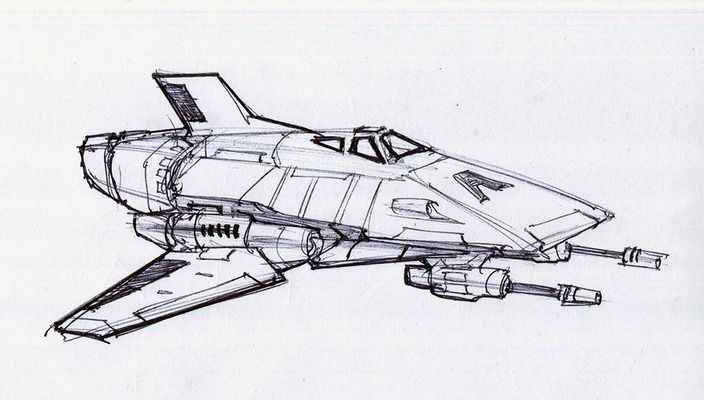
\includegraphics[height=4cm, width=7cm]{a.jpg}\\
\end{center}

\section{Découpage des tâches}

\paragraph{Création des niveaux :}
La conception des niveaux dans lesquels évoluera le joueur se decoupe en plusieurs parties : La création du terrain et des objets provoquant des collisions, la définition de la zone jouable et l'application des textures.

\paragraph{Gameplay :}
Le gameplay est l'expérience du joueur, c'est-à-dire le controle du vaisseaux, l'intelligence artificielle, l'interface utilisateur, les règles du jeu ainsi que les différents modes de jeu proposés dans Flight Arena.
Le jeu devra être jouable au clavier.

\paragraph{L'Intelligence Artificielle :}
Pour occuper le joueur solitaire dépourvu de connection internet, une intelligence artificielle controlera des vaisseaux pour les diriger vers les ennemis et faire feu.

\paragraph{Script :}
Composé de programmation à l'état pur, cette partie contrôle le fonctionnement du jeu

\paragraph{Gestion des données :}
Il s'agit de créer une base de données pour stocker tous les éléments du jeu. Elle devra aussi faciliter la gestion des différents objets utilisés par le joueur( par exemples les munitions ou le nombre de points de vie restants).

\paragraph{Moteur graphique :}
Le moteur graphique devra gérer l'affichage des textures, de l'environnement et des animations. Il devra aussi intéragir avec le joueur( changement de position de la caméra par exemple)

\paragraph{Moteur physique :}
Ce moteur devra détecter les collisions entre les différents éléments du jeu, calculer la trajectoire des vaisseaux et tous les effets entrainés par les actions du joueur.

\paragraph{Réseaux :}
Comme le dit le proverbe: Plus on est de fous, plus on rit ! Nous proposerons donc aux joueurs de jouer en réseau. Cela présente deux avantages: faire des lan endiablées et alonger la durée de vie du jeu.

\paragraph{Site web :}
Ce site web sera une facade de notre projet, donc une partie importante du marketing. Il présentera les membres du groupe, l'avancée de notre projet, le cahier des charges, les rapports de soutenance, la version finale du projet( lorsque celle-ci sera disponible),...

\paragraph{Finalisation du projet :}
Tout le monde n'a pas forcément Unity installé.Nous proposerons donc un executable d'installation et de désinstallation du jeu ainsi qu'une version CD.

\chapter{L'aspect utilitaire et économique}

Nous utiliserons comme langage de programmation le C\#.

\section{Logiciels et utilitaires}

Voici la liste des logiciels et utilitaires que nous utiliserons :\\

\begin{tabular}{|c|c|c|}
\hline
Logiciel & Fonction & Coût\\
\hline
Unity & Moteur graphique & 0 \euro\\
\hline
Visual Studio & Code & 428,29 \euro\\
\hline
Blender & Modélisation 3D & 0 \euro\\
\hline
Adobe Photoshop & Textures et images & 699 \euro\\
\hline
Adobe Dreamweaver & Site internet & 470 \euro\\
\hline
Audacity & Son & 0 \euro\\
\hline
Git et SourceTree & Partage du programme & 0 \euro\\
\hline
Tex Live & Rédaction & 0 \euro\\
\hline
\multicolumn{2}{|c|}{Total } & 1597,29 \euro\\
\hline
\end{tabular}\\
\\

\begin{center}
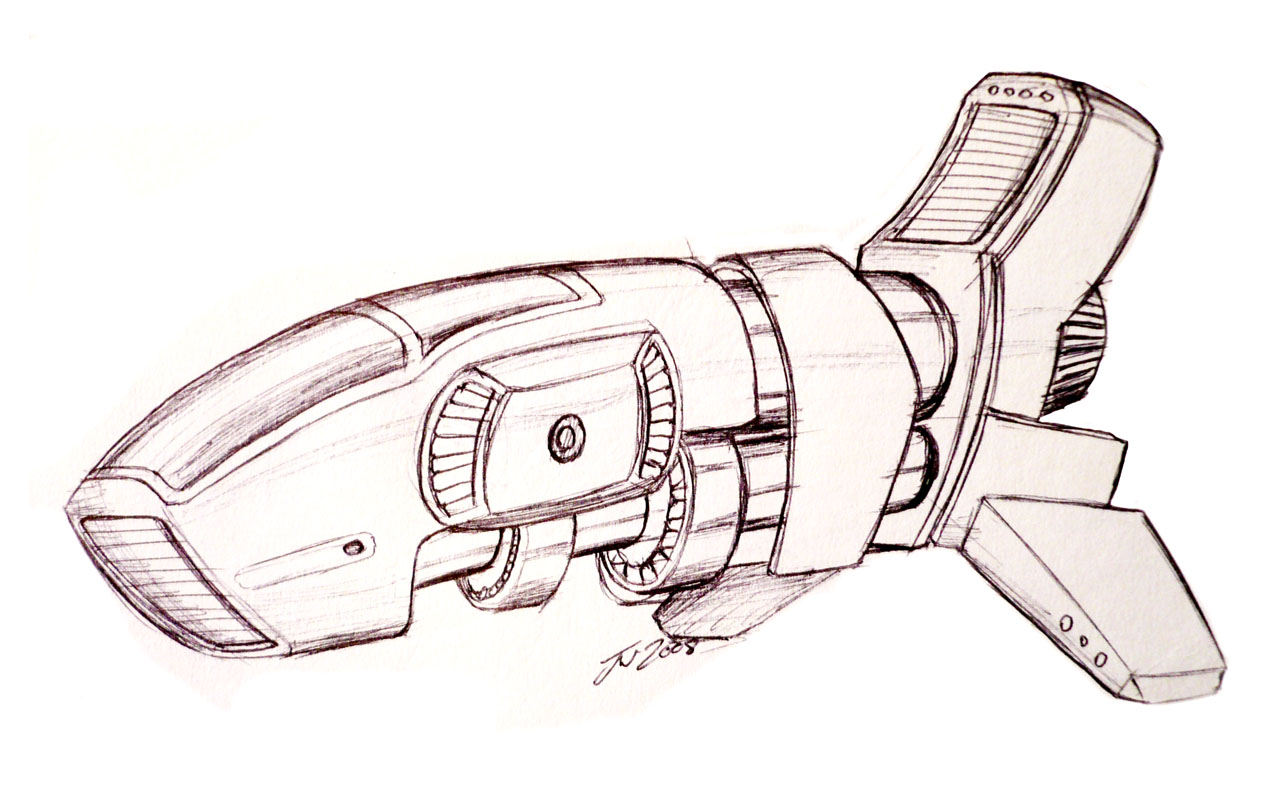
\includegraphics[height=4cm, width=6.4cm]{b.jpg}
\end{center}

\section{Ordinateurs et outils}

Comme ordinateurs, nous utilisons :\\

\begin{tabular}{|c|c|c|}
\hline
Propriétaire & Ordinateur & Coût\\
\hline
%Nikolas Miletic & Predator G7 & 1700 \euro\\
%\hline
Arthur Remaud & HP Pavilion 15-n054sf & 600 \euro\\
\hline
Vincent Rospini-Clerici & Samsung série 3 & 500 \euro\\
\hline
Guillaume Rebut & Ordinateur fixe assemblé & 1000 \euro\\
\hline
\multicolumn{2}{|c|}{Total } & 2100 \euro\\
\hline
\end{tabular}\\

Nous utliserons de plus les ordinateurs mis à disposition en salle machine pour travailler ensemble.\\

Le coût total du projet s'élève donc à environ 3697,29 \euro.

\chapter{Déroulement du projet et répartition du travail}

Dans les tableaux ci-dessous est décrit la répartition des tâches et leur avancement pour chaque soutenance.\\

$\times$ : commencé\\
$\times \times$ : avancé\\
$\times \times \times$ : terminé

\section{Première soutenance}

\begin{tabular}{|*{4}{p{2cm}|}}
\hline
Tâches & Arthur Remaud & Vincent Rospini Cleric & Guillaume Rebut \\
\hline
Gameplay & $ \times $ & & $ \times $ \\
\hline
Création de niveaux & & $ \times $ & $ \times $ \\
\hline
I.A & & & \\
\hline
Script & $ \times $ & & \\
\hline
Gestion des données & & &\\
\hline
Moteur graphique & & $ \times \times $ & \\
\hline
Moteur physique & $ \times \times $ & & $ \times \times $ \\
\hline
Réseaux & & & \\
\hline
Site web & & & \\
\hline
\end{tabular}\\

\section{Deuxième soutenance}

\begin{tabular}{|*{4}{p{2cm}|}}
\hline
Tâches & Arthur Remaud & Vincent Rospini Clerici & Guillaume Rebut \\
\hline
Gameplay & $ \times \times \times $ & & $ \times \times \times $ \\
\hline
Création de niveaux & & $ \times \times  $ & $ \times \times $ \\
\hline
I.A & $ \times $ & & $ \times $ \\
\hline
Script & $ \times \times $ & & \\
\hline
Gestion des données & $ \times \times $ & $ \times \times $ & \\
\hline
Moteur graphique & & $ \times \times $ & \\
\hline
Moteur physique & $ \times \times\times  $ & & $ \times \times \times $ \\
\hline
Réseaux & & $ \times $ & $ \times $ \\
\hline
Site web & & $ \times \times $ &  \\
\hline
\end{tabular}\\

\section{Soutenance finale}

\begin{tabular}{|*{4}{p{2cm}|}}
\hline
Tâches & Arthur Remaud & Vincent Rospini Clerici & Guillaume Rebut \\
\hline
Gameplay & $ \times \times \times $ & & $ \times \times \times $ \\
\hline
Création de niveaux & & $ \times \times \times $ & $ \times \times \times $ \\
\hline
I.A & $ \times \times \times $ & & $ \times \times \times $ \\
\hline
Script & $ \times \times \times $ & & \\
\hline
Gestion des données & $ \times \times\times  $ & $ \times \times\times  $ & \\
\hline
Moteur graphique & & $ \times \times \times $ & \\
\hline
Moteur physique & $ \times \times \times $ & & $ \times \times \times $ \\
\hline
Réseaux & & $ \times \times \times$  & $ \times \times \times $ \\
\hline
Site web & & $ \times \times \times $ & \\
\hline
\end{tabular}\\


\chapter{Objectifs de ce projet}

L'idée d'un projet de groupe amène à envisager une multitude de caractéristiques à prendre en compte, aussi bien dans le domaine de l'enseignement que dans celui du travail. Il permet notamment de faire face à des situations d'autonomie, qui s'avèrent nécessaires à son avancement. Il s'agit de se montrer indépendant, et de réaliser son travail individuel essentiel à l'avancement du projet. Le temps de réalisation est tout aussi important, puisqu'il faut également prendre en compte le fait que le temps imparti est de six mois, ce qui laisse à penser que cette idée de réalisation n'est absolument pas à prendre à la légère, mais qu'il faut, au contraire, être conscient de la quantité de réflexion (et donc de travail!) requise à l'aboutissement, ou, du moins, à un résultat satisfaisant du projet au terme de ce semestre.

Un tel projet permet de concrétiser et de mettre en évidence un exemple de mode de programmation propice au développement du software (en l’occurrence, un jeu) dont nous aurons l'opportunité – voire l'obligation – de mettre en pratique dans le futur.\\

Même s'il s'agit d'acquérir de l'expérience vis-à-vis de soi, et de comprendre ce système de fonctionnement de manière individuelle et autonome, il ne faut pas négliger le fait que ce projet devra être réalisé en groupe. Dans le monde du travail, la coopération est une recette nécessaire à l'aboutissement des projets. La répartition des tâches est une réflexion sur laquelle il faut faire appel aux compétences propres à chaque membre, afin de pouvoir travailler de manière optimale. Il s'agira là d'optimiser le travail, et de progresser de la manière la plus efficace possible.

La communication est également essentielle, car il nous faudra adapter la qualité de travail en fonction du développement de chacun, et de toujours avoir une longueur d'avance sur l'avancement total, afin de ne pas être dépassés, et, si possible, de prendre de l'avance dans l'optique de pouvoir aboutir avant la fin du temps imparti. Il est question d'acquisition d'expérience par une méthode qui n'est pas forcément accessible à chacun, et le cadre scolaire d'EPITA nous permet de nous mettre en situation réelle afin de pouvoir envisager le futur qui nous est préparé d'une manière plus aisée et de ne pas être pris au dépourvu dans ce cadre.\\ \\ \\ \\ \\ \\ \\ \\ \\ \\ \\

\begin{center}
\centering
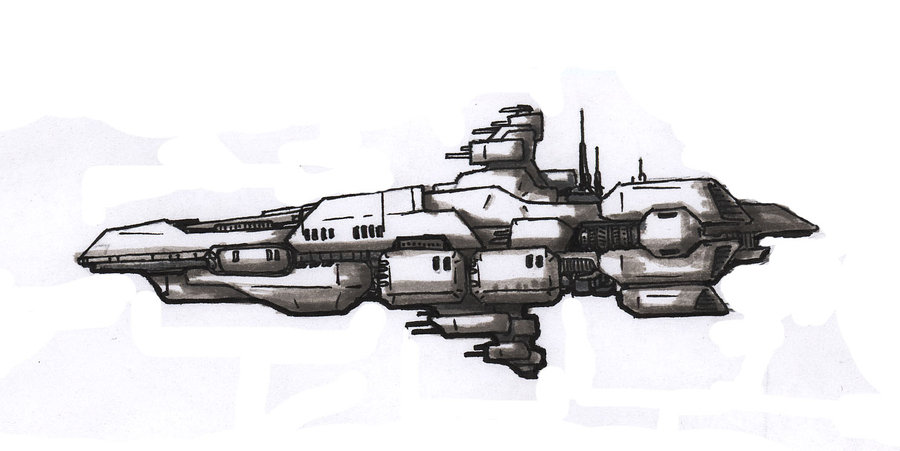
\includegraphics[height=3cm, width=6cm]{c.jpg}
\end{center}

\chapter{Conclusion}

Ainsi commença le long périple de ces quatre aventuriers de l'extrême. Le groupe mr cube se lança à corps perdus dans cette lourde tâche qui leur tenait pourtant à c\oe{}ur. Ils savaient qu'ils devaient faire de nombreux sacrifices pour arriver à leurs fins : manger des pizzas froides, boire des hectolitres de caféine et autres calamités. Durant des mois ils passèrent tout leur temps libre, à suer sang et eau pour atteindre leur rêve ultime : leurs noms sur les crédits de fin du jeu.
\\ \\ \\ \\ \\ \\ \\
\begin{center}

\includegraphics[height=4cm, width=4cm]{vaisseux_petit.png}
\end{center}

\end{document}